\documentclass[border=3pt]{standalone}
% Preâmbulo compartilhado pelos diagramas TikZ da aula 6 de Navegação (Implementação do Wavefront)
\usepackage[T1]{fontenc}
\usepackage[utf8]{inputenc}
\usepackage{lmodern}
\usepackage{amsmath}
\usepackage{xcolor}
\usepackage{tikz}
\usetikzlibrary{arrows.meta,angles,quotes,decorations.pathmorphing,decorations.pathreplacing,calc,
                positioning,shapes.geometric,shapes.misc,backgrounds,fit,
                math}

% Paleta (mesma dos SVGs originais)
\definecolor{dblue}{HTML}{2A5B8C}
\definecolor{dorange}{HTML}{B3541E}
\definecolor{dgreen}{HTML}{4A7C59}
\definecolor{dred}{HTML}{9C4B4B}
\definecolor{dcream}{HTML}{F4F1EA}
\definecolor{dshade}{HTML}{DDD7C9}

% Função gaussiana (não normalizada por padrão de escala visual)
\pgfmathdeclarefunction{gauss}{3}{%
  \pgfmathparse{1/(#3*sqrt(2*pi))*exp(-((#1-#2)^2)/(2*#3^2))}%
}

% Estilos comuns (prefixo d... para não colidir com chaves internas do pgf)
\tikzset{
  >={Stealth[length=2mm]},
  dguide/.style={gray!55, dashed, line width=0.4pt},
  daxis/.style={gray!60, line width=0.7pt, ->},
  dbody/.style={fill=black!3, draw=black!80, line width=1pt},
  dacc/.style={draw=dblue, line width=1pt},
  dlbl/.style={black!55, font=\small},
  dsub/.style={black!45, font=\footnotesize},
  dstate/.style={circle, draw=black!80, fill=dcream, line width=1pt,
                 minimum size=17mm, font=\large, inner sep=1pt},
  dobs/.style={circle, draw=black!80, fill=dshade, line width=1pt,
               minimum size=14mm, font=\large, inner sep=1pt},
  dbox/.style={rounded corners=2pt, draw=black!80, fill=dcream, line width=1pt,
               align=center, inner sep=6pt},
  dop/.style={circle, draw=black!80, fill=white, line width=1pt,
              minimum size=6mm, inner sep=0pt, font=\small},
  dtrans/.style={->, dblue, line width=1pt},
  dmeas/.style={->, dorange, line width=1pt},
  dcurve/.style={line width=1pt, dblue},
  dcurveb/.style={line width=1.4pt, dorange},
}

\begin{document}
\hyphenpenalty=10000 \exhyphenpenalty=10000 \tolerance=9999 \emergencystretch=3em
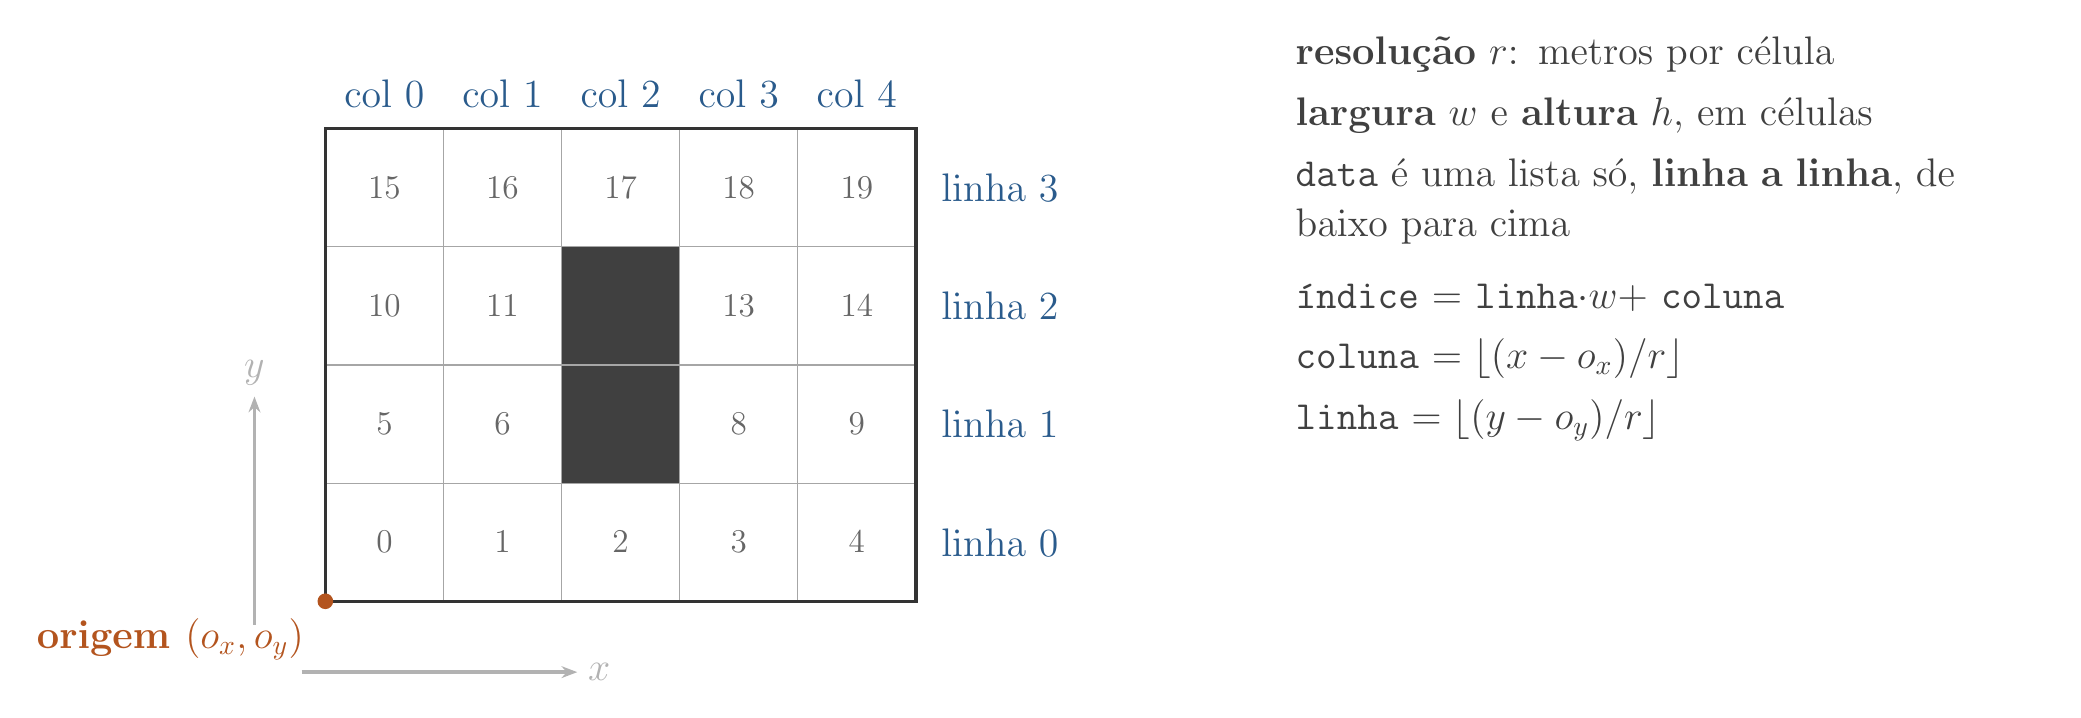
\begin{tikzpicture}[x=1cm,y=1cm]
\draw[fill=white, draw=black!35] (0.00,0.00) rectangle ++(1.50,1.50);
\node[font=\large, black!60] at (0.75,0.75) {0};
\draw[fill=white, draw=black!35] (1.50,0.00) rectangle ++(1.50,1.50);
\node[font=\large, black!60] at (2.25,0.75) {1};
\draw[fill=white, draw=black!35] (3.00,0.00) rectangle ++(1.50,1.50);
\node[font=\large, black!60] at (3.75,0.75) {2};
\draw[fill=white, draw=black!35] (4.50,0.00) rectangle ++(1.50,1.50);
\node[font=\large, black!60] at (5.25,0.75) {3};
\draw[fill=white, draw=black!35] (6.00,0.00) rectangle ++(1.50,1.50);
\node[font=\large, black!60] at (6.75,0.75) {4};
\draw[fill=white, draw=black!35] (0.00,1.50) rectangle ++(1.50,1.50);
\node[font=\large, black!60] at (0.75,2.25) {5};
\draw[fill=white, draw=black!35] (1.50,1.50) rectangle ++(1.50,1.50);
\node[font=\large, black!60] at (2.25,2.25) {6};
\draw[fill=black!75, draw=black!35] (3.00,1.50) rectangle ++(1.50,1.50);
\draw[fill=white, draw=black!35] (4.50,1.50) rectangle ++(1.50,1.50);
\node[font=\large, black!60] at (5.25,2.25) {8};
\draw[fill=white, draw=black!35] (6.00,1.50) rectangle ++(1.50,1.50);
\node[font=\large, black!60] at (6.75,2.25) {9};
\draw[fill=white, draw=black!35] (0.00,3.00) rectangle ++(1.50,1.50);
\node[font=\large, black!60] at (0.75,3.75) {10};
\draw[fill=white, draw=black!35] (1.50,3.00) rectangle ++(1.50,1.50);
\node[font=\large, black!60] at (2.25,3.75) {11};
\draw[fill=black!75, draw=black!35] (3.00,3.00) rectangle ++(1.50,1.50);
\draw[fill=white, draw=black!35] (4.50,3.00) rectangle ++(1.50,1.50);
\node[font=\large, black!60] at (5.25,3.75) {13};
\draw[fill=white, draw=black!35] (6.00,3.00) rectangle ++(1.50,1.50);
\node[font=\large, black!60] at (6.75,3.75) {14};
\draw[fill=white, draw=black!35] (0.00,4.50) rectangle ++(1.50,1.50);
\node[font=\large, black!60] at (0.75,5.25) {15};
\draw[fill=white, draw=black!35] (1.50,4.50) rectangle ++(1.50,1.50);
\node[font=\large, black!60] at (2.25,5.25) {16};
\draw[fill=white, draw=black!35] (3.00,4.50) rectangle ++(1.50,1.50);
\node[font=\large, black!60] at (3.75,5.25) {17};
\draw[fill=white, draw=black!35] (4.50,4.50) rectangle ++(1.50,1.50);
\node[font=\large, black!60] at (5.25,5.25) {18};
\draw[fill=white, draw=black!35] (6.00,4.50) rectangle ++(1.50,1.50);
\node[font=\large, black!60] at (6.75,5.25) {19};
\draw[black!80, line width=1.2pt] (0,0) rectangle (7.50,6.00);
\node[circle, fill=dorange, inner sep=2pt] at (0,0) {};
\node[font=\Large\bfseries, dorange, anchor=north east] at (-0.15,-0.1) {origem $(o_x, o_y)$};
\draw[daxis, line width=1.2pt, ->] (-0.3,-0.9) -- (3.2,-0.9) node[right, font=\Large] {$x$};
\draw[daxis, line width=1.2pt, ->] (-0.9,-0.3) -- (-0.9,2.6) node[above, font=\Large] {$y$};
\node[font=\Large, dblue] at (0.75,6.45) {col 0};
\node[font=\Large, dblue] at (2.25,6.45) {col 1};
\node[font=\Large, dblue] at (3.75,6.45) {col 2};
\node[font=\Large, dblue] at (5.25,6.45) {col 3};
\node[font=\Large, dblue] at (6.75,6.45) {col 4};
\node[font=\Large, dblue, anchor=west] at (7.70,0.75) {linha 0};
\node[font=\Large, dblue, anchor=west] at (7.70,2.25) {linha 1};
\node[font=\Large, dblue, anchor=west] at (7.70,3.75) {linha 2};
\node[font=\Large, dblue, anchor=west] at (7.70,5.25) {linha 3};
\node[font=\Large, black!75, anchor=west, text width=9.5cm, align=left] at (12.2,4.6) {\textbf{resolução} $r$: metros por célula\\[4pt] \textbf{largura} $w$ e \textbf{altura} $h$, em células\\[4pt] \texttt{data} é uma lista só, \textbf{linha a linha}, de baixo para cima\\[8pt] \texttt{índice} $=$ \texttt{linha}$\cdot w +$ \texttt{coluna}\\[4pt] \texttt{coluna} $=\lfloor (x-o_x)/r \rfloor$\\[4pt] \texttt{linha} $=\lfloor (y-o_y)/r \rfloor$};
\end{tikzpicture}
\end{document}
